\documentclass[tikz]{standalone}
\usepackage{pgfplots}
\pgfplotsset{compat=1.15}
\usepackage{mathrsfs}
\usetikzlibrary{arrows,calc}
\usepackage{tkz-euclide}
\pagestyle{empty}

\definecolor{AngleClr}{rgb}{0,0.39215686274509803,0}
\definecolor{ShapeClr}{rgb}{0.6,0.2,0}

\begin{document}

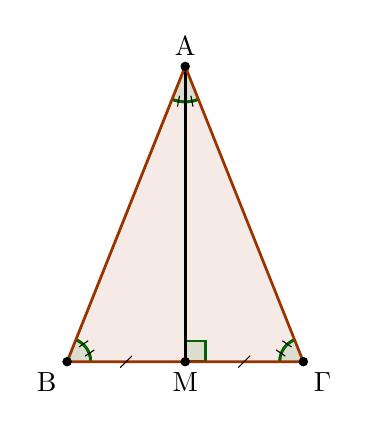
\begin{tikzpicture}[scale=.75]
\tkzSetUpLine[line width=1pt,color=black]
\tkzSetUpPoint[fill=black]

\tkzDefPoints{0/0/B,2/5/A,4/0/C,2/0/M}


\tkzFillPolygon[fill=ShapeClr,fill opacity=0.1](A,B,C)
\tkzFillAngles[fill=AngleClr,size=.4,fill opacity=0.1](C,B,A A,C,B)
\tkzMarkAngles[line width=1pt,size=.4,color=AngleClr](C,B,A A,C,B)
\tkzMarkAngles[mark=||,mksize=2,line width=1pt,size=.4,color=AngleClr](C,B,A  A,C,B)


\tkzFillAngle[fill=AngleClr,size=.6,fill opacity=0.1](B,A,C)
\tkzMarkAngle[line width=1pt,color=AngleClr,size=.6](B,A,C)
\tkzMarkAngles[mark=|,mksize=2,line width=1pt,size=.6,color=AngleClr](B,A,M M,A,C)

\tkzMarkRightAngle[line width=1pt, size=.35,color=AngleClr,fill=AngleClr,fill opacity=0.1](A,M,C)

\tkzDrawSegment[line width=1pt,color=black](A,M)

\tkzDrawPolygon[color=ShapeClr](A,B,C)
\tkzDrawPoints[size=3](A,B,C,M)
\tkzLabelPoint[above](A){$\rm A$}
\tkzLabelPoint[below left](B){$\rm B$}
\tkzLabelPoint[below right](C){$\rm \Gamma$}
\tkzLabelPoint[below](M){$\rm M$}

\tkzMarkSegments[mark=s|,size=3](B,M M,C)

\end{tikzpicture}
\end{document}
